\documentclass{ltjsarticle}
\usepackage{amsmath}
\usepackage{amssymb}
\usepackage{ascmac}
\usepackage[dvipdfmx]{graphicx}
\usepackage{tabularx}
\usepackage[colorlinks=true, allcolors=blue]{hyperref}
\usepackage{fancybox}
\usepackage{tikz}
\usepackage{subcaption}
\usetikzlibrary{shapes,arrows}

\begin{document}

\title{102. 深層学習の適用方法(物体検知)}
\author{秋葉洋哉}
\maketitle

\section{物体検知}
\subsection{概要}
深層学習を用いた物体検知の研究の流れは、徐々に難易度を上げてきた。その流れは以下のとおりである。
\begin{itemize}
  \item 分類(Classification) : 画像に対して複数のクラスラベルを出力
  \item 物体検知(Object Detection) : 画像中の物体の位置を推定 (Bounding Box)
  \item 意味領域分割(Semantic Segmentation) : 各ピクセルに対して単一のクラスラベルを出力
  \item 個体領域分割(Instance Segmentation) : 各ピクセルかつ個体毎に対して単一のクラスラベルを出力
\end{itemize}

\begin{figure}[htbp]
  \centering
  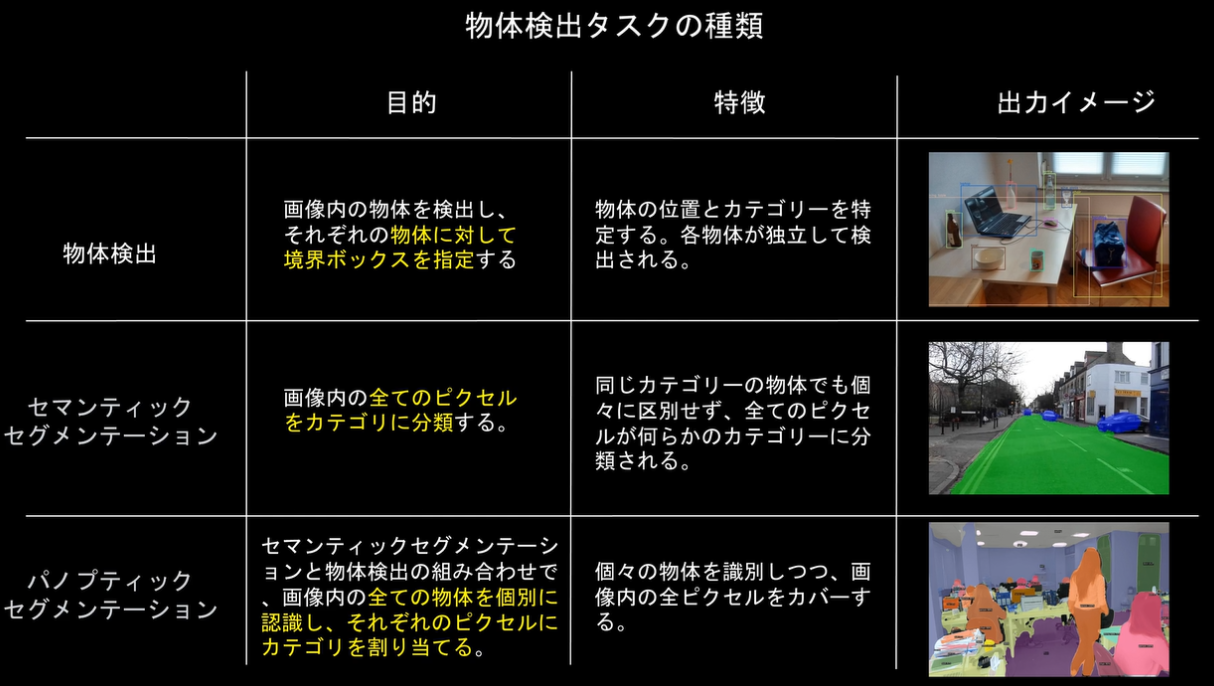
\includegraphics[width=13cm]{./capture/Matrix.png}
  \caption{物体検出タスクの種類}
  \label{fig:Matrix}
\end{figure}

物体検出では、BoundingBoxとConfidenceの2種が同時に出力される。BoundingBoxは物体の位置を示し、Confidenceはその物体が存在する確信度を示す。

\subsection{データセット}
物体検知に用いられるデータセットは、VOC12, ILSVRC17, MS COCO18, OICOD18などがある。
\par
VOC12(Visual Object Classes)は20クラス、Train+Valは11,540枚、Box/画像(1画像当たりの物体数)=2.4 であり、(PASCAL VOC Detection Challenge)というコンペティションで使用されていた。VOC12のGround TruthのBBに関する情報は<xmin>, <ymin>, <xmax>, <ymax>の四つのタグが示す長方形で与えられる。
\par
ILSVRC17(ImageNet Large Scale Visual Recognition Challenge)は200クラス、Train+Valは476,668枚、Box/画像(1画像当たりの物体数)=1.1 であり、(ImageNet Large Scale Visual Recognition Challenge)というコンペティションで使用されていた。ImageNetは、画像認識のためのデータセットであり、ILSVRCはそのサブセットである。
\par
MS COCO18(Microsoft Common Objects in Context)は80クラス、Train+Valは123,287枚、Box/画像(1画像当たりの物体数)=7.3 であり、(Microsoft Common Objects in Context)というコンペティションで使用されていた。
\par
OICOD18(Open Images Challenge Detection)は500クラス、Train+Valは1,743,042枚、Box/画像(1画像当たりの物体数)=7.0 であり、(Open Images Challenge Detection)というコンペティションで使用されていた。Open Images V4は、6000クラス以上/900万枚以上の画像を含むデータセットであり、そのサブセットがOICOD18である。
\par
Box/画像(1画像当たりの物体数)は、小さいほどアイコン的な映りであり、日常感とは異なる。大きいほど日常感に近い映りであり部分的な重なりも見られるようになる。
\par
どのような物体検知モデルを作成したいかを考える時は、Box/画像(1画像当たりの物体数)とクラス数を考慮する必要がある(図\ref{fig:BoxFig_Class})。

\begin{figure}[htbp]
  \centering
  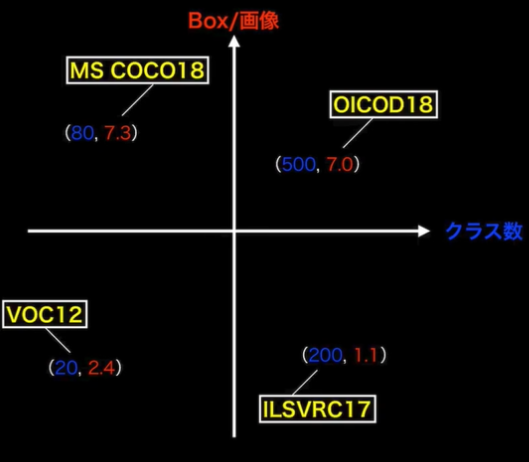
\includegraphics[width=8cm]{./capture/BoxFig_Class.png}
  \caption{代表的データセットのポジショニングマップ}
  \label{fig:BoxFig_Class}
\end{figure}

\subsection{評価指標}
混合行列(図\ref{fig:Confusion_Matrix})を確認すると、一般的に予測する際の評価指標は、精度(Precision), 再現率(Recall), 正解率(Accuracy)が用いられる。これらの指標は、Thresholdによって変化する。クラス分類では、Thresholdに応じて、分類されるクラスが変化するが、物体検出では、Thresholdに応じて、BoundingBoxの数が変化する(図\ref{fig:Threshold})。
\begin{figure}[htbp]
  \centering
  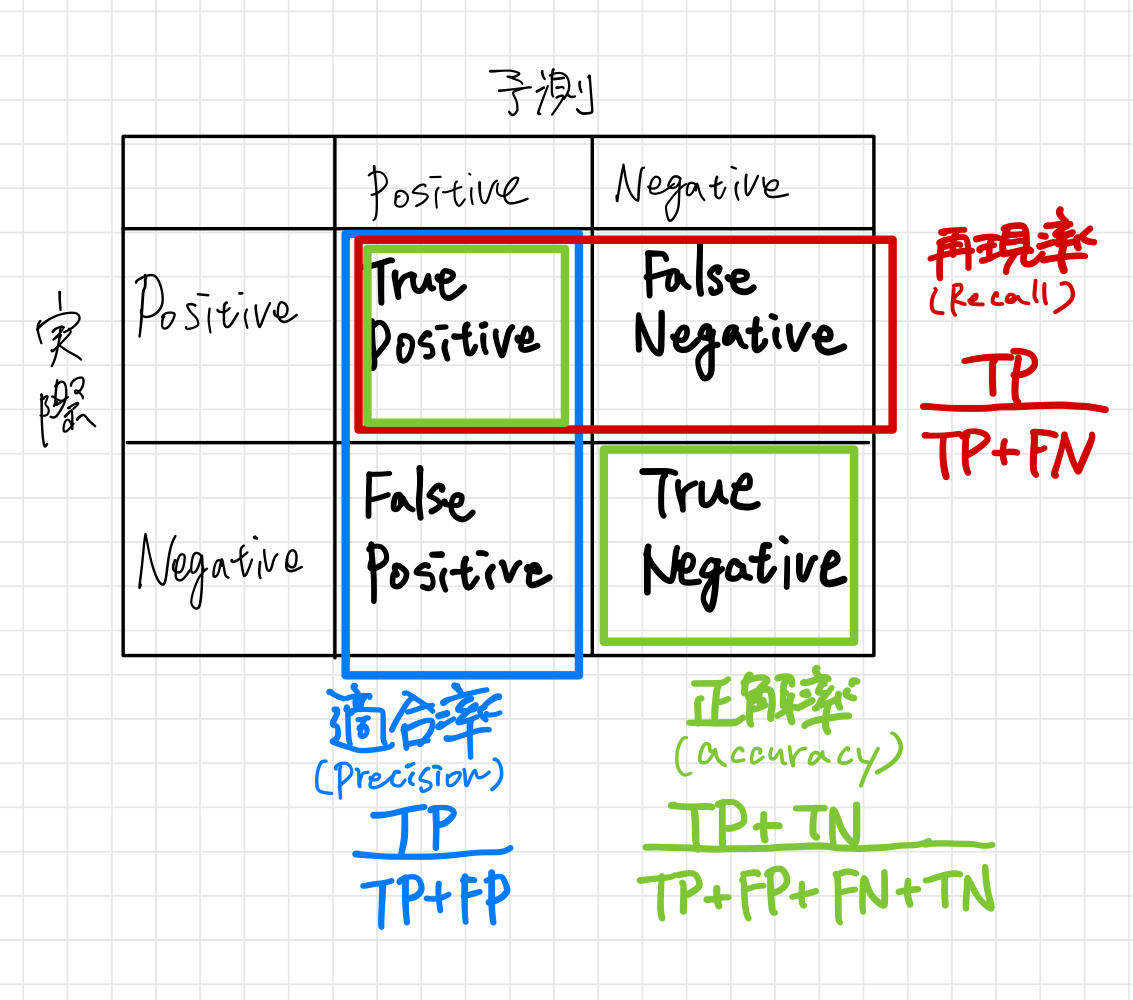
\includegraphics[width=10cm]{./capture/Confusion_Matrix.png}
  \caption{混合行列(復習)}
  \label{fig:Confusion_Matrix}
\end{figure}
\begin{figure}[htbp]
  \centering
  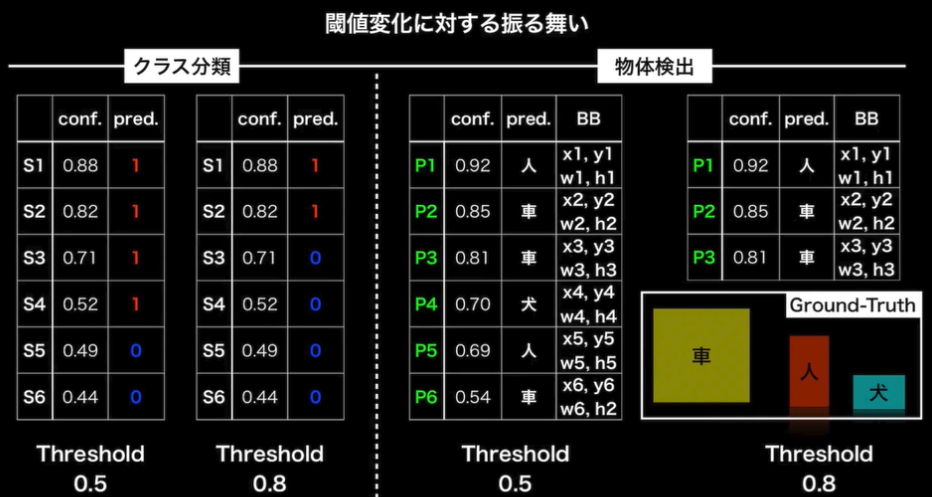
\includegraphics[width=10cm]{./capture/Threshold.png}
  \caption{Thresholdの変化に対するクラス分類と物体検出の違い}
  \label{fig:Threshold}
\end{figure}
\par
物体検知において精度は、予測で出力したBBoxの数に対する、正解のBBoxの数の割合であり、予測のBBoxが真のBBox数よりも多い場合、精度の高い順にTPとみなし、残りはFPとみなすことで求まる。つまり、予測のBBoxが多いほど精度は下がる。一方再現率は、真のBBoxの数に対する、予測で出力したBBoxの数の割合であり、予測のBBox数が真のBBox数よりも少ない場合、その分をFNとみなすことで求まる。つまり、予測のBBoxが少ないほど再現率は下がる。
\par
このPrecision-RecallをThresholdの関数としてプロットしたものをPrecision-Recall curveと呼ぶ。また、Precision-Recall curveの下の面積を求めたものをAP(Average Precision)と呼ぶ。APは、物体検知の性能を評価する指標であり、APが高いほど性能が良いとされる。
\par
物体検知の評価指標には、AP(平均適合率)とmAP(平均適合率)がある。APは、クラスごとのAPの平均値であり、mAPは、全クラスのAPの平均値である。mAPは、物体検知の性能を評価する指標であり、mAPが高いほど性能が良いとされる(図\ref{fig:AP_mAP})。

\begin{figure}[htbp]
  \centering
  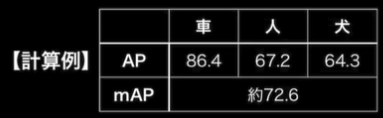
\includegraphics[width=6cm]{./capture/AP_mAP.png}
  \caption{APとmAPの違い}
  \label{fig:AP_mAP}
\end{figure}

IoU(Intersection over Union)は、真のBoundingBoxと予測のBoundingBoxの重なり具合を示す指標であり、IoUが0.5以上のBoundingBoxを正解とする場合が多い。IoUは以下で定義される。
\begin{align}
  \text{IoU} &= \frac{(\text{Area of Overlap})}{(\text{Area of Union})}\\
  &= \frac{TP}{TP+FP+FN}
\end{align}
これを図で示したのが図\ref{fig:IoU}, 図\ref{fig:IoU_example}である。物体検知では、ConfidenceとIoUの2つの指標を用いて評価することが多い。
\begin{figure}[htbp]
  \centering
  \begin{subfigure}[b]{0.45\textwidth}
    \centering
    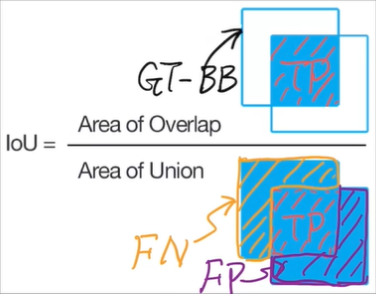
\includegraphics[width=\textwidth]{./capture/IoU.png}
    \caption{IoUの定義}
    \label{fig:IoU}
  \end{subfigure}
  \hfill
  \begin{subfigure}[b]{0.45\textwidth}
    \centering
    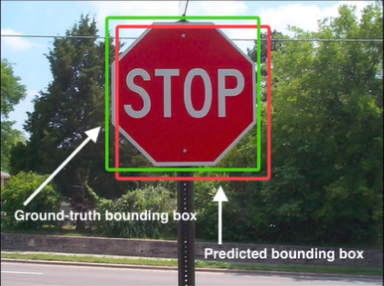
\includegraphics[width=\textwidth]{./capture/IoU_example.png}
    \caption{IoUの例}
    \label{fig:IoU_example}
  \end{subfigure}
  \caption{IoUについて}
\end{figure}

\subsection{検出速度}
物体検知のモデルの性能を評価する際には、検出速度も重要な指標である。検出速度は、FPS(Frame Per Second)で表され、1秒間に何枚の画像を処理できるかを示す。検出速度は、モデルの複雑さや画像サイズによって変化する。検出速度が速いほど、リアルタイムでの物体検知に適していると言える。
横軸にFPS, 縦軸にmAPを取ったグラフや、横軸にinference time, 縦軸にmAPを取ったグラフを作成することで、検出速度と性能のトレードオフを可視化することができる(図\ref{fig:Speed_Accuracy})。
\begin{figure}[htbp]
  \centering
  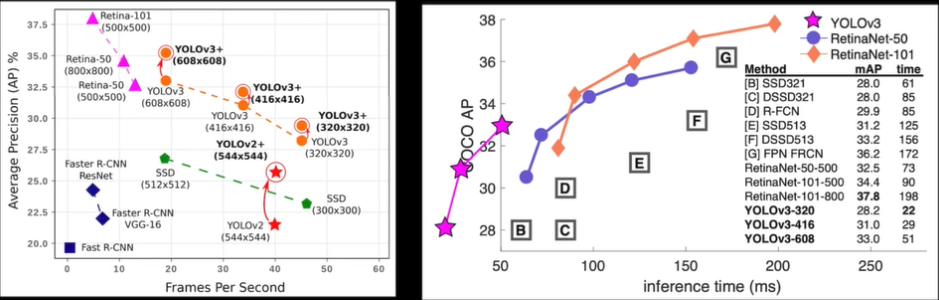
\includegraphics[width=14cm]{./capture/Speed_Acuracy.png}
  \caption{検出速度と性能のトレードオフ}
  \label{fig:Speed_Accuracy}
\end{figure}

\clearpage
\section{深層学習以降の物体検知}
物体検知のフレームワークは深層学習の進化に伴って同時に進化した。メカニズムに基づき大きく分けて2つに分類できる。
\begin{itemize}
  \item 2段階検出(2-stage detection) : 物体の候補領域を検出し、その領域に対して物体のクラスと位置を別々に推定する (相対的に精度が高いが、計算量が多く、推論も遅い)
  \item 1段階検出(1-stage detection) : 物体のクラスと位置を同時に推定する (相対的に精度が低いが、計算量が少なく、推論も速い)
\end{itemize}
2段階検出は、RCNN, FastRCNN, FasterRCNN, MaskRCNNなどがある。1段階検出は、SSD, YOLO, RetinaNet, DetecorNet, CornerNetなどがある。リアルタイムで検出する場合は、1段階検出が適している。

\clearpage
\section{SSD(Single Shot MultiBox Detector)}
SSDは、1段階検出の代表的なモデルであり、物体のクラスと位置を同時に推定する。
その方法は、以下の通りである。
\begin{enumerate}
  \item 画像を入力する。
  \item 画像上に適当にDefault Boxを配置する。
  \item Default Boxを変形し、検出したい物体のクラスとConf.を推定する。
\end{enumerate}
SSDはVGG16というネットワークをベースにしており、VGG16の最後の畳み込み層を利用して特徴マップを取得する(VGG16の16はConvolution層の数である)。

\subsection{SSDのアーキテクチャ}
SSDのアーキテクチャは、以下の通りである。
\begin{enumerate}
  \item 入力 : 画像を入力。入力サイズに応じてSSD300, SSD512などと表記される。
  \item 隠れ層 : VGG16の10層目に対応するConv層(38$\times$38のConv層),や、VGG16のFC(Fully Connected)層2層に対応する層 (FC6, FC7層) をConv層に変更して、様々なサイズの特徴マップを取得する。
  \item 出力 : Default Box(クラス数+4(場所に関する項))を出力する。1つの特徴マップに対して、k個のDefault Boxを出力する($k\times$(クラス数+4))ため、特徴マップのサイズが$m\times n$の場合合計で、($k\times$(クラス数+4))$mn$個のDefault Boxを配置する。
\end{enumerate}
特徴マップの解像度が高いほど、小さな物体を検出することができ、特徴マップの解像度が低いほど、大きな物体を検出することができるため、様々な解像度の特徴マップを用いることで、様々なサイズの物体を検出することができる。
\par
VOCデータセットでは、クラス数20に背景クラスが追加されるため、クラス数21に対して、合計の出力は、8,732$\times$(21+4)個となる。
\par
このように多数のDefault Boxを用意したことで、1つの物体しか映っていなくても、複数のPredicted-BBoxが表示されることになってしまう。この問題を解決するために、Non-Maximum Suppression(NMS)という手法が用いられる。NMSでは、Predicted-BBox同士のIoUを計算し、閾値を超えた場合1つを残して他を削除することで、1つの物体に対して1つのPredicted-BBoxを残す。
\par
また、多数のDefault Boxを用意することで、背景を示すPredicted-BBoxに対して、物体を示すPredicted-BBoxの比率がとても小さくなってしまう。この問題を解決するために、Hard Negative Miningという手法が用いられる。Hard Negative Miningでは、背景を示すPredicted-BBoxと、物体を示すPredicted-BBoxの比率が1:1 ~ 3:1までになるように制約を課すことで、背景を示すPredicted-BBoxの比率を減らす。

\subsection{損失関数}
SSDの損失関数は、以下の通りである。
\begin{align}
  L &= L_{\text{loc}} + L_{\text{conf}} + L_{\text{hardneg}}\\
  L_{\text{loc}} &= \sum_{i}^{N} \sum_{j\in Pos}^{N} \text{SmoothL1}(l_{ij} - \hat{g}_{ij})\\
  L_{\text{conf}} &= -\sum_{i}^{N} \text{log}(\hat{c}_{ij})\\
  L_{\text{hardneg}} &= -\sum_{i}^{N} \text{log}(\hat{c}_{ij})
\end{align}
ここで、$L_{\text{loc}}$は、位置に関する損失関数、$L_{\text{conf}}$は、クラスに関する損失関数、$L_{\text{hardneg}}$は、背景を示すPredicted-BBoxに対する損失関数である。また、$l_{ij}$は、Predicted-BBoxの位置、$\hat{g}_{ij}$は、Ground Truthの位置、$\hat{c}_{ij}$は、Predicted-BBoxのクラス、$Pos$は、Positive Sampleを示す。

\clearpage
\section{Semantic Segmentation}
\subsection{概要}
Semantic Segmentationは、画像の各ピクセルに対して単一のクラスラベルを出力するタスクである。画像のピクセルごとにクラスを推定するため、画像全体に対してクラスラベルを付与することができる。
\par
Semantic Segmentationは、FCN(Fully Convolutional Network)やU-Net, SegNet, DeepLabなどのモデルが提案されている。これらのモデルは、畳み込みニューラルネットワークを用いて画像の各ピクセルに対してクラスラベルを推定する。
\par
ネットワーク内でクラスを分類するためには、解像度を落とす必要がある。一方で、各ピクセル毎のクラスを求めるためには、出力時に元の画像の解像度に戻さなければならない。そのため、画像の解像度を落としてから、再び元の解像度に戻す、Up-samplingという処理が必要となる。

\subsection{FCN(Fully Convolutional Network)}
FCNは、Semantic Segmentationのアーキテクチャモデルの一つであり、VGG16における最後のFC層をすべてConv.層に置き換え、すべての層が畳み込み層で構成されたネットワークである。このような変換を用いることで、出力としてヒートマップのようなものが得られることになる。
\par
Semantic Segmentationでは、最終的に元画像と同一の解像度の画像を出力するため、FCNによって全結合層を畳み込み層に変換することで、Up-Sampling前の無駄な処理を省くことができる。
\par
FCNの特徴として、最終的に全結合層を有さないため、入力画像の解像度は任意のサイズであっても良い。

\begin{itembox}{Poolingの重要性}
  Semantic Segmentationにおいて、画像の解像度をもとに戻すために、Up-samplingが必要ということが分かったが、そもそもPoolingしなければUp-samplingも必要ないと思うかもしれない。
  \par
  まず、機械が正しく、犬であるか、猫であるかを認識するためには、受容野にある程度の大きさが必要である。受容野を広げる例としては、深いConv.層を用いる、Pooling+Stlideを行う、Dilated Convolutionなどが挙げられる。
  \par
  1つ目の深いConv.層を用いる方法は、受容野を広げることができるが、計算量が多くなるという問題がある。2つ目のPooling+Stlideを行う方法は、計算量を多くせずに、受容野を広げることができる。
  \par
  よって、Poolingは、受容野を広げ、その画像に対する特徴を抽出するために重要であるので、欠かすことができない処理になる。
  \par
  3つ目のDilated Convolutionは、後ほど詳しく説明する。
\end{itembox}

\subsection{Up-sampling}
Up-samplingは、画像の解像度を元に戻す処理であり、画像の解像度を落とすPoolingとは逆の処理である。Up-samplingの一つとして、DeconvolutionやTransposed convolution という仕組みが用いられる。

\subsubsection{Deconvolution}
Deconvolutionは、以下の手順で行われる。
\begin{enumerate}
  \item Kernel size, padding, strideの各値を指定する
  \item 特徴マップのpixel間隔をstrideだけ空ける
  \item 特徴マップの周りに、(kernel size - 1) - padding だけ余白を作る
  \item 畳み込み演算を行う
\end{enumerate}
この手順を示した画像が、図\ref{fig:Up-sampling}である。
\begin{figure}[htbp]
  \centering
  \includegraphics[width=7cm]{./capture/Up-sampling.png}
  \caption{Up-samplingの概要}
  \label{fig:Up-sampling}
\end{figure}
この手法は、解像度を基に戻すことができるが、Poolingで失われた情報が復元されるわけではない。
Poolingによって失われた輪郭のようなローカルな情報は、Skip Connectionを用いて、解像度の高いPooling層と結合することで、復元していくことになる (図\ref{Up-sampling_prediction})。
\begin{figure}[htbp]
  \centering
  \includegraphics[width=10cm]{./capture/Up-sampling_prediction.png}
  \caption{Up-samplingとSkip Connectionの結合}
  \label{Up-sampling_prediction}
\end{figure}

\subsubsection{Unpooling}
Unpoolingは、Poolingで画像の解像度を落とした際に失われた情報を復元するための処理である。Unpoolingは、Pooling時に記憶しておいた位置情報を用いて、元の画像の解像度に戻す処理である。Unpoolingの手法として、以下の2つがある。
\begin{itemize}
  \item Max Unpooling : Pooling時にMax値を取った位置を記憶しておき、その位置にMax値を配置する
  \item Nearest Unpooling : Pooling時にMax値を取った位置を記憶しておき、その位置に最も近い値を配置する
\end{itemize}
Max Unpoolingは、Pooling時にMax値を取った位置を記憶しておくため、元の画像の解像度に戻す際に、Max値を配置する。一方、Nearest Unpoolingは、Pooling時にMax値を取った位置を記憶しておくため、元の画像の解像度に戻す際に、その位置に最も近い値を配置する。

\subsection{U-Net}
U-Netは、Semantic Segmentationのモデルの一つであり、Encoder-Decoder構造を持つ。U-Netは、以下の特徴を持つ。
\begin{itemize}
  \item Encoder-Decoder構造 : 特徴マップをEncoderで抽出し、Decoderで元の解像度に戻す
  \item Skip Connection : 同じ段階のEncoderの特徴マップとDecoderの特徴マップを結合することで、ローカルな情報を復元する
  \item 損失関数 : クロスエントロピー誤差を用いる
\end{itemize}
U-Netは、FCNの要素ごとの特徴マップの結合 (Element-wise addition)を行うわけではなく、チャネル方向で特徴マップを結合する (Concatenation) 。このような結合方法を用いることで、FCNとは異なる方法でローカルな情報を復元することができる(図\ref{fig:U-Net})。
\begin{figure}[htbp]
  \centering
  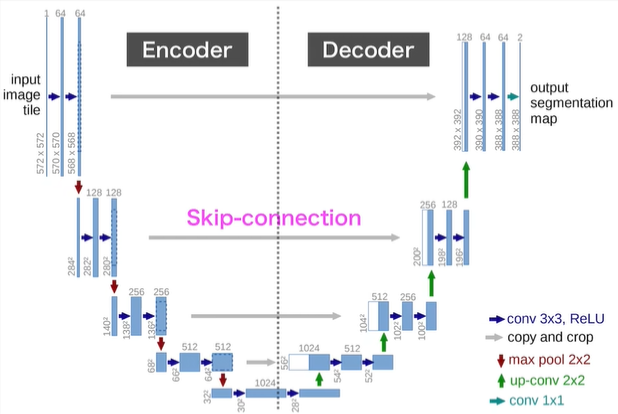
\includegraphics[width=10cm]{./capture/U-Net.png}
  \caption{U-Netのアーキテクチャ}
  \label{fig:U-Net}
\end{figure}

\subsection{Dilated Convolution}
Dilated Convolutionは、畳み込み演算において、フィルタの間に空白を入れることで、Poolingを用いずに受容野を広げる手法である。図\ref{fig:Dilated_Convolution}にDilated Convolutionの例を示す。
\begin{figure}[htbp]
  \centering
  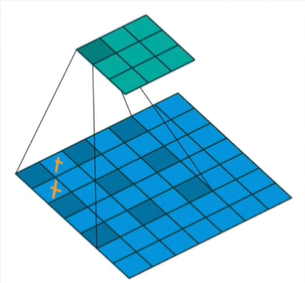
\includegraphics[width=7cm]{./capture/Dilated_Convolution.png}
  \caption{Dilated Convolutionの例: 3×3カーネルを用いて、5×5の畳み込みを行うことで、結果7×7の出力を得ることができる。Inputの濃くなっている部分がフィルタの適用ピクセルになる。隙間(rate)を広くすることで、より広い受容野を得ることができる。}
  \label{fig:Dilated_Convolution}
\end{figure}



\clearpage
\section{Instance Segmentation}
Instance Segmentationは、Semantic Segmentationの拡張であり、各ピクセルに対して単一のクラスラベルを出力するだけでなく、個体毎にクラスラベルを出力するタスクである。つまり、同じクラスであっても、異なる個体に対して異なるクラスラベルを出力する。

\subsection{Mask R-CNN}
Mask R-CNNは、物体検知とInstance Segmentationを同時に行うモデルである。
物体検出では、物体の同定(identification: 画像の中で物体がどこにあるのか)と、物体認識/分類(classification: 物体が何であるのか)を行う。
また、Instance Segmentationでは、物体の同定と、物体の領域を示すマスクを出力する。
この2つの作業を同時に行うことで、Mask R-CNNは、画像の中で物体がどこにあり、その物体が何であるのか、そしてさらにその物体の領域を示すマスクを出力することができる。
\par
Mask R-CNNは、R-CNNをベースとしている。R-CNNは、物体検出のみを行うモデルであり、物体の同定と物体認識/分類を行う。R-CNNでは、以下の手順で物体検出を行う。
\begin{enumerate}
  \item 画像を入力する
  \item 画像から物体の関心領域(ROI: Region of Interest)を抽出して、類似する領域をグルーピングする
  \item 各ROIに対して、画像の大きさを揃え、CNNを用いて特徴量を求める
  \item 特徴量を用いて、SVMで学習を行い、物体のクラスを推定する
\end{enumerate}
R-CNNは、物体検出の精度は高いが、計算量が多く、推論も遅いという問題があった。この問題を解決するために、Fast R-CNNが提案された。Fast R-CNNでは、ROI毎にCNNに通さず、画像全体をCNNに通す(ROI Pooling)ことで、計算量を削減し、推論速度を向上させた。
\par
さらに、Faster R-CNNが提案された。Faster R-CNNでは、物体の関心領域(ROI)を抽出をも、CNNで行うことで、より高速に物体検出を行うことができるようになった。
\par
Mask R-CNNは、Faster R-CNNにセグメンテーションの機能を追加したモデルである。
Mask R-CNNでは、画像全体ではなく、物体検出の結果として得られた領域についてのみセグメンテーションを行うことで、Faster R-CNNよりも複雑で細かい領域だけでなく、より高速に出力を得ることができる。

\subsubsection{ROI Pooling}
ROI Poolingは、Mask R-CNNにおいて用いられた手法で、Fast/Faster R-CNNでも用いられる手法である。
ROI Poolingは、畳み込み処理後の特徴マップから、画像全体を固定サイズの特徴マップとして抽出する。

\subsection{FCOS}
FCOS(Fully Convolutional One-Stage Object Detection)は、物体検出を行うモデルであり、アンカーフリーのモデルである。
\par
アンカーとはPredicted-BBoxの位置を決定するための基準となるBBoxであり、SSDなどで用いられる。アンカーフリーのモデルでは、その基準となるアンカーを用いずに、物体の位置を推定する。具体的には、特徴マップの各ピクセルのうち、Ground TruthのBBoxに入っていれば、そのピクセルを物体の中心として、Positiveサンプルと判定する。
\par
アンカーを用いる場合、アンカーのサイズ・アスペクト比・数などのハイパーパラメータによって、精度が大きく変動したり、小さな物体に対しての判別が難しくなったり、ネガポジ比率が悪くなるという問題があった。FCOSでは、アンカーを用いないことでこれらの問題を解決する。
\par
FCOSは、FPN(Feature Pyramid Network)というアーキテクチャを採用(図\ref{FCOS_Architecture})し、異なる解像度の特徴マップを組み合わせることで、様々なサイズの物体を検出することができる。
\begin{figure}[htbp]
  \centering
  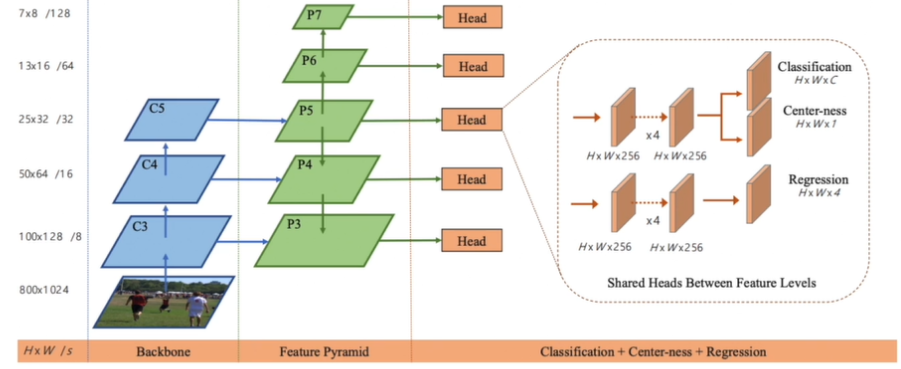
\includegraphics[width=10cm]{./capture/FCOS_Architecture.png}
  \caption{FCOSのアーキテクチャ}
  \label{FCOS_Architecture}
\end{figure}
\par
FCOSで学習する内容は
\begin{itemize}
  \item 物体のクラス (Classification)
  \item 物体の位置 (Regression)
  \item 物体の中心 (Centerness)
\end{itemize}
である。
FCOSでは、Centernessという概念を導入する。Centernessは、以下の式で定義される。
\begin{align}
  \text{Centerness} = \sqrt{\frac{\text{min}(l, r)}{\text{max}(l, r)} \times \frac{\text{min}(t, b)}{\text{max}(t, b)}}
\end{align}
ここで、$l, r, t, b$は、Predicted-BBoxの中心から左端、右端、上端、下端までの長さを表す。
Centernessは中心から離れた位置に、低品質のPredicted-BBoxが多数生成される課題にたいして、物体中心に近い位置に高品質のPredicted-BBoxを生成するための指標である。




\clearpage
\paragraph{参考文献}
\begin{enumerate}
  \item 岡谷貴之/深層学習 改訂第2版 [機械学習プロフェッショナルシリーズ]/ 講談社サイエンティフィク/ 2022-01-17
  \item 1日1分 E資格問題 No.23「FCOS」 \url{https://e-shikaku-doujou.com/fcos}
\end{enumerate}

\newpage
\end{document}